% Template for PLoS
% Version 1.0 January 2009
%
% To compile to pdf, run:
% latex plos.template
% bibtex plos.template
% latex plos.template
% latex plos.template
% dvipdf plos.template

\documentclass[11pt]{article}

% amsmath package, useful for mathematical formulas
\usepackage{amsmath}
% amssymb package, useful for mathematical symbols
\usepackage{amssymb}
\usepackage{booktabs}
% graphicx package, useful for including eps and pdf graphics
% include graphics with the command \includegraphics
\usepackage{graphicx}

% cite package, to clean up citations in the main text. Do not remove.
\usepackage{cite}

\usepackage{color} 

% Use doublespacing - comment out for single spacing
%\usepackage{setspace} 
%\doublespacing


% Text layout
\topmargin 0.0cm
\oddsidemargin 0.5cm
\evensidemargin 0.5cm
\textwidth 16cm 
\textheight 21cm

% Bold the 'Figure #' in the caption and separate it with a period
% Captions will be left justified
\usepackage[labelfont=bf,labelsep=period,justification=raggedright]{caption}

% Use the PLoS provided bibtex style
\bibliographystyle{plos2009}

% Remove brackets from numbering in List of References
\makeatletter
\renewcommand{\@biblabel}[1]{\quad#1.}
\makeatother


% Leave date blank
\date{}

\pagestyle{myheadings}
%% ** EDIT HERE **
\usepackage{enumerate}
\usepackage{multirow} 
\usepackage{url}
\usepackage{xr} %for cross-referencing
%% ** EDIT HERE **
%% PLEASE INCLUDE ALL MACROS BELOW
\newtheorem{algorithm}{Algorithm}
\newtheorem{proposition}{Proposition}
\newtheorem{restateproposition}{Proposition}
\newtheorem{lemma}{Lemma}
\newtheorem{corollary}{Corollary}
\newtheorem{result}{Result}
\newtheorem{note}{Note}
\newtheorem{definition}{Definition}

\def\lfdr{\text{lfdr}}
\def\lfsr{\text{lfsr}}
\def\x{\mbf{x}}
\def\y{\mbf{y}}
\def\e{\mbf{e}}
\def\g{\mbf{g}}
\def\p{p}
\def\Yb{\hat{Y}_1^{\text{BAYES}}}
\def\Xperp{X_{1 \perp 0}}
\def\Pperp{P_{1 \perp 0}}
\def\Pperpb{\Pperp^{\text{B}}}
\def \hatd { \widehat{ d } }
\def \dhatin {\hatd^{\mbox{\tiny IN}}}
\def \dhatsw {\hatd^{\mbox{\tiny SW}}}
\def \mvn{\text{MVN}}
\def\mn{\text{MN}}
\def \iw{\text{W}^{-1}}
\def \fp {fastPHASE\ }
\def\bhat{\hat{\beta}}
\def\shat{\hat{s}}
\def\var{\rm Var}
\def\mvr{\text{BMVR}}
\def\bfuni{\text{BF}_\text{uni}}
\def\one{\mbf{1}}
\def\zero{\mbf{0}}
\def\hall{H_{\text{all}}}
\def\pall{\p_{\text{all}}}
\def\bfall{\text{BF}_\text{all}}
\def\bfav{\text{BF}_\text{av}}
\def\gall{\gamma_\text{all}}
\def\limbfall{\bfall^\rightarrow}
\def\limbfav{\bfav^\rightarrow}
\def\limbfgamma{\BF_\gamma^\rightarrow}
\def\sxx{S_{xx}}
\def\syy{S_{yy}}
\def\vyy{V_{yy}}
\def\vyx{V_{yx}}
\def\vxx{{V_{xx}}}
\def\rss{\text{\rm RSS}}
\def\dss{\text{\rm $\Delta$SS}}
\def\U{U}
\def\D{D}
\def\I{I}
\def\luu{L_{UU}}
\def\indep{\perp}
\newcommand{\mbf}[1]{\mbox{\boldmath$#1$}} % true mathbf works in math
                                % mode too
\newcommand\height{{\it height}}
\newcommand\weight{{\it weight}}
\def\BF{\text{BF}}


%% END MACROS SECTION
\externaldocument{plos_one_rev1_suppinfo}

\begin{document}

% Title must be 150 characters or less
\begin{flushleft}
{\Large
\textbf{False Discovery Rates: A New Deal}
}
% Insert Author names, affiliations and corresponding author email.
\\
Matthew Stephens$^{1*}$, 
\\
\bf{1} Department of Statistics and Department of Human Genetics, University of Chicago, Chicago, IL, USA
\\
$\ast$ E-mail: Corresponding mstephens@uchicago.edu
\end{flushleft}

% Please keep the abstract between 250 and 300 words
\section*{Abstract}

% Please keep the Author Summary between 150 and 200 words
% Use first person. PLoS ONE authors please skip this step. 
% Author Summary not valid for PLoS ONE submissions.   
%\section*{Author Summary}

\section*{Introduction}

Since its introduction in 19xx by Benjamini and Hochberg 
\cite{bh:xx}, the ``False Discovery Rate" (FDR) has quickly established itself
as a key concept in modern statistics. 
%, and the primary tool by which most practitioners handle large-scale multiple testing.
Here we consider one setting in which FDR-based methods are widely used:
an experimenter has measured a large numbers of ``effects", each with an associated
measurement precision (standard error), 
and the goal is to identify which of the effects we can declare to be non-zero (with some prescribed level of confidence).
This setting arises commonly in many areas of statistics, and particularly in genomics applications.
For example, in genomics
a common goal is to identify ``differentially-expressed genes" -- that is, genes
whose mean expression (activity) level differs in two conditions. 


%Let $\mu^0_j$ and $\mu^1_j$ denote the mean expression 
%of gene $j$ ($j=1,\dots,J$) in the two conditions, and define $\beta_j:= \mu^0_j - \mu^1_j$ to be the difference. Typically expression
%measurements are made on only a small number of
%samples in each condition - sometimes as few as one
%sample in each condition. Thus the error in estimates
%of $\mu^0_j$ and $\mu^1_j$ is appreciable, and the error
%in estimates of $\beta_j$ still greater.
%

Many tools have been developed for this problem \cite{}, and several are widely used.
Here we argue that these existing tools have sub-optimal features that can be improved on, at least in some circumstances.
In particular we argue that existing tools i) fail to take proper account of variations in the measurement precision of different effects;
ii) make, implicitly, unrealistic assumptions about the distribution of the non-zero effects. We provide methods
to address these problems, implemented in an R package {\tt ashr} (short for ``Adaptive Shrinkage") and demonstrate that these methods can lead to a substantial reduction in estimated FDRs (or, equivalently,
a substantial increase in the number of discoveries at a given FDR).  

Although we motivate our tools by FDR, we are providing generic tools for shrinkage, and
these could be useful in settings such as wavelets.
The potential for shrinkage-based estimation to
address the multiple comparisons problems tackled by the FDR
has been highlighted
previously, including Greenland and Robins (1991),
Efron (2008) and Gelman et al (2012). [Note, check also Louis, JASA, 1984] 


The initial goal of the ASH (Adaptive SHrinkage) project is to provide simple, generic, and flexible methods to derive ``shrinkage-based" estimates and credible intervals for unknown quantities $\beta=(\beta_1,\dots,\beta_J)$, given only estimates of those quantities ($\bhat=(\bhat_1,\dots, \bhat_J)$) and their corresponding estimated standard errors ($s=(s_1,\dots,s_J)$). 

Although shrinkage-based estimation can be motivated in various ways, our key goal here is to combine information across the multiple measurements $j=1,\dots,J$ to improve inference for each individual $\beta_j$. By improved inference, we mean both
improved average accuracy of point estimates, which is
the traditional focus of shrinkage-based methods, \emph{and} improved assessments of uncertainty. 

By ``adaptive" shrinkage we 
have two key properties in mind. First, the appropriate amount of shrinkage is determined from the data, rather than being pre-specified. Second, the amount of shrinkage undergone by each $\bhat_j$ will depend on the standard error $s_j$: measurements with high standard error will undergo more shrinkage than measurements with low standard error.

Given that shrinkage estimation is widely recognized as a powerful tool, there are surprisingly few software packages for performing the simplest type of shrinkage estimation considered here. (There are more packages for the more complex setting of covariance estimation, where shrinkage is perhaps still more important.)
The only package we have found that provides anything similar
to the functionality provided here is mixfdr (Muralidharan). Compared with mixfdr, the key features of ashr are that it
i) focuses on allowing for variation in the standard deviation of each observation; ii) constrains the underlying density to be unimodal (and possibly symmetric).
NOTE: should emphasize these differences in the examples.

As an important special case, these methods address the "multiple comparisons" setting, where interest usually focuses on which $\beta_j$ can be confidently inferred to be non-zero. Such problems are usually tackled by computing a $p$ value for each $j$, often by applying a $t$ test to $\bhat_j/s_j$,
and then applying a generic procedure, such as that of Benjamini 
and Hochberg (1995?) or Storey (2001?), designed to control or
estimate the false discovery rate (FDR) or the positive FDR (Storey, 2001?). In essence we aim to provide analagous
generic methods that work directly with two numbers for each 
measurement $(\bhat_j,s_j$), rather than a single number (e.g.~ the $p$ value, or $t$ statistic). Working with these two numbers has two important benefits: first, it permits estimation and not only testing; second, the 
uncertainty in each measurement $\bhat_j$ can be more fully accounted for, reducing the impact of ``high-noise" measurements (large $s_j$) that can reduce the effectiveness of a standard FDR analysis. 

\def\df{df}
\def\FDR{\text{FDR}}
\def\fdr{\text{lfdr}}

 \section*{Methods}
 
 \subsection*{Notation, and existing methods}
 
Suppose that we are interested in the values of $J$ ``effects" $\beta_j$ ($j=1,\dots,J$). In some contexts our interest may focus on which of the $\beta_j$ are ``significantly" different from zero, whereas in other contexts our interest may focus on estimating their values; the methods described here are suited to both these contexts.
 We assume that we have obtained data $D_1,\dots,D_J$ that provide independent estimates $\bhat_1,\dots,\bhat_J$ of these effects,
 with corresponding (estimated) standard errors $\shat_1,\dots,\shat_J$. For our purposes, these estimates and standard errors could be obtained from the data
 using any method, provided they (approximately) satisfy 
 \begin{equation} \label{eqn:betahat-t}
 \bhat_j \big{|} \, \beta_j, \shat_j \sim t_\nu(\beta_j,\shat_j),
 \end{equation}
for some known degrees of freedom (\df) $\nu$, where $t_\nu(\mu,\sigma)$ denotes the generalized $t$ distribution on $\nu$ \df, with mean $\mu$ and scale parameter $\sigma$. (Equivalently, $(\bhat_j-\beta_j)/\shat_j \big{|} \, \beta_j \sim t_\nu$, where $t_\nu$ denotes the standard $t$ distribution on $\nu$ \df.)
In the special case $\nu \rightarrow \infty$ this includes the situation where the $\bhat$ can be considered normally distributed:
  \begin{equation} \label{eqn:betahat-norm}
 \bhat_j  \big{|} \, \beta_j, \shat_j \sim N(\beta_j,\shat^2_j).
 \end{equation}
 Assuming (\ref{eqn:betahat-t}), the $t$-statistics defined by
 \begin{equation} 
 t_j:=\bhat_j/\shat_j
 \end{equation}
 have a $t_\nu$ distribution under the $j$th null hypothesis $H_j:\beta_j=0$, and this fact can be used to compute a $p$ value $p_j$ testing $H_j$.

One nice feature of the False Discovery Rate (FDR) is that Frequentist and Bayesian definitions are closely aligned.
Here we provide Bayesian definitions, and refer the reader to \cite{storey.03}, particularly his Theorem 1,  for connections with frequentist definitions.
The (tail) FDR at threshold $T$ is defined as
\begin{equation}
\FDR(T) := \Pr(\text{$H_j$ false} | t_j \geq T).
\end{equation}
The local FDR at $t$ is defined \cite{efron} as
\begin{equation}
\fdr(t) := \Pr(\text{$H_j$ is false} | t_j = t).
\end{equation}
The local FDR is perhaps more relevant than the tail FDR, but less widely used because
it is harder to estimate (density estimation is harder than tail area estimation). 
The $q$ value for observation $j$ is defined \cite{storey.03} as:
\begin{equation}
q_j := \FDR(t_j).
\end{equation}
That is, the $q$ value is the FDR if we reject the null for all observations that are at least as significant as $j$.

One standard genomics analysis pipeline is to take the $p$ values $p_1,\dots,p_J$ and convert them to (estimated) $q$ values $q_1,\dots,q_J$
 using the R package {\tt qvalue}. A graphical description of how {\tt qvalue} works is given in Figure \ref{}. 




\subsection*{Problems with existing methods}

 There are two issues with this approach that I would like to address here. The first is that it really does not take proper account of the measurement errors. To see this, consider an example where half the measurements are quite precise, and the other half are really, really, poor. Intuitively, the poor measurements tell us nothing, and any sane analysis should effectively ignore them. However, in a standard FDR-type analysis, these poor measurements add ``noise" and affect estimated FDRs. This is because the $p$ values from the poor measurements will be effectively uniformly distributed, and some will be significant at any given threshold. 
 
Illustration (Figure).

Note that the problem could be reduced by discarding measurements that are too noisy. However,
note limitation of this.

The second issue is that directly modeling the p values, or z scores, say via non-parametric methods, 
can lead to unrealistic distributions being fitted. Put another way, because z scores are the result of adding noise to some
distribution, the range of distributions they can take is limited Using entirely non-parametric methods loses this information.
The solution is to model beta hat as a convolution of some distribution g and an error component.

Illustration (Figure).


 
 
 %(See Discussion for ideas on how our methods may be applicable more generally; for example if, in place of $\shat_j$, we have a $p$ value testing $\beta_j=0$.)
 
 In outline, we use a hierarchical model to combine information across measurements, with the aim of improving both accuracy and precision of estimates. 
 Specifically we assume that the effects $\beta_j$ are independent and identically distributed from some unknown distribution $g(\cdot)$,
 \begin{equation} \label{eqn:beta}
 \beta_j \sim g(\cdot),
 \end{equation}
 where $g$ will be estimated from
 the data.  Our methods make the following key assumptions, which distinguish them from most previous work in this area:
   \begin{enumerate}
  \item[A1:] The distribution $g(\cdot)$ is unimodal. (We assume here that the mode is at 0, although 
this could be relaxed.)  
 \item[A2:] The likelihood $L(\beta_j) := p(D_j | \beta_j)$ can be approximated by a normal likelihood,
 \begin{equation} \label{eqn:lik}
 \hat{L}_j(\beta_j) \propto \exp[-0.5(\beta_j-\bhat_j)^2/\shat_j^2].
 \end{equation}
%which, in light of (\ref{eqn:betahat}), is equivalent to
 % \begin{equation} \label{eqn:lik2}
% L(\beta_j) \propto p(\bhat_j | \beta_j, \shat_j).
 %\end{equation}
 \end{enumerate}
 
 \subsubsection*{Discussion on Assumptions}
 
Although the unimodal assumption, A1, will not apply to all situations, we argue that it will be reasonable in many practical contexts. 
For example, in contexts where interest focusses on which $\beta_j$ differ from zero, which suggests that ``$\beta_j=0$" is a plausible null hypothesis,  
it seems reasonable to expect that ``$\beta_j$ very near 0" is also plausible, and that the distribution of the effects will be unimodal about 0. 
Alternatively, we can motivate A1 by its effect on point estimates, which is to ``shrink" the estimates towards the mode - 
such shrinkage is desirable from several standpoints for improving estimation accuracy. 
Note that assumption A1 relates to the distribution of {\it all} effects, and not only the {\it detectable} effects (i.e.~those that are significantly different from zero). It is very likely that the distribution of {\it detectable} non-zero effects will be multimodal, with one mode for detectable positive effects and another for detectable negative effects, and A1 does not contradict this.

Interestingly, although the unimodal assumption A1 seems natural, much previous related work on estimating False Discovery Rates  
has assumed, either explicitly or implicitly, that the effect sizes are multimodal (see Results for more details). 
In contrast, almost all analogous work in large-scale regression assumes
a unimodal prior distribution for the effect sizes, common choices being the spike and slab, Laplace, $t$, normal-gamma, normal-inverse-gamma, or horseshoe priors.
One of our aims here is to emphasize potential benefits of also making the unimodal assumption in the FDR context.

Assumption A2 can derived from (\ref{eqn:betahat}) plus a couple of other assumptions. Specifically, assume that a) $\bhat_j, \shat_j$ contain most of the information about $\beta_j$ in the data $D_j$ (i.e. they are ``approximately sufficient" for $D_j$) and that b) $\shat_j$ alone contains little information about $\beta_j$. The former (a) suggests the approximation $\hat{L}_j(\beta_j) \propto p(\bhat_j, \shat_j | \beta) = p(\bhat | \beta, \shat_j) p(\shat_j | \beta)$, while the latter (b) suggests assuming that $p(\shat_j|\beta_j)$ does not depend on $\beta_j$. Putting these two together yields $\hat{L}_j(\beta_j) \propto p(\bhat_j | \beta, \shat_j)$, which, with (\ref{eqn:betahat}),  implies A2. If $\bhat_j, \shat_j$ are not sufficient for $D_j$ then there is some loss of efficiency in making this approximation, but all Bayesian inferences remain valid provided they are interpreted as conditional on $\bhat_j,\shat_j$, rather than conditional on $D_j$. See \cite{johnson.xx} and \cite{wakefield.xx} for more general discussion and examples of Bayesian inference based on summary statistics. 

Alternatively A2 could be considered definitional for $\bhat_j,\shat_j$: that is, choose $\bhat_j,\shat_j$ such that A2 holds. 

While Assumption A2 has parallels with approaches like \cite{efron, cai?} that model the $Z$ scores $Z_j = \bhat_j/\shat_j$ as normally distributed under the null, 
there is an important difference: here, observations with a large $\shat_j$ have an essentially flat likelihood (\ref{eqn:lik}), and so do not affect inference for
other parameters, whereas when modeling the $Z$ scores directly, observations with large $\shat_j$ produce $Z$ scores with an $N(0,1)$ distribution that {\it do} affect inference. 
Because of this the likelihood-based approach can take better account of the informativeness of each measurement, as illustrated in Results below.

%The choice of normal likelihood seems natural, and indeed it can be motivated in multiple ways. For example, we can write $p(\bhat_j, \shat_j | \beta_j) = p(\bhat_j | \shat_j, \beta_j)p(\shat_j | \beta_j)$. Now, if we are willing to assume that $\shat_j$ alone contains no information about $\beta_j$, or equivalently that $p(\shat_j | \beta_j)$ does not depend on $\beta_j$, then $L(\beta_j) \propto p(\bhat_j | \shat_j, \beta_j)$, and if $\bhat_j | \shat_j, \beta_j \sim N(\beta_j, \shat_j^2)$, as is often asymptotically the case, then we obtain the likelihood (**) above.

\subsubsection*{Implementing the Unimodal assumption}
 
In practice, we implement the unimodal assumption (A1) by assuming a parametric finite mixture for $g$, 
\begin{equation} \label{eqn:g}
g(\cdot; \pi) = \pi_0 \delta_0(\cdot) + \sum_{k=1}^K \pi_k f_k(\cdot) 
\end{equation}
where $\delta_0(\cdot)$ denotes a point mass at 0, $\pi=(\pi_0,\dots,\pi_K)$ are mixture proportions to be estimated (with $\pi_j \geq 0, \sum_j \pi_j=1$), and $f_k$ are pre-specified 
component distributions with one of the following forms: 
\begin{enumerate}[i)]
\item $f_k(\cdot) = N(\cdot; 0, \sigma^2_k)$
\item $f_k(\cdot) = U[\cdot; -a_k,a_k]$
\item $f_k(\cdot) = U[\cdot; -a_k,0] \text{ or } U[\cdot; 0,a_k]$,
\end{enumerate}
where $N(\cdot; 0,\sigma^2)$ denotes the density of a normal distribution with mean 0 and variance $\sigma^2$ and
$U[\cdot; a,b]$ denotes the density of a uniform distribution on $[a,b]$.
That is, the non-zero effects are modeled as either i) a mixture of zero-centered normal distributions; ii) a mixture of zero-centered uniform distributions;
or iii) a mixture of ``zero-anchored" uniform distributions, which have one end of their range at 0. These approaches closely mirror approaches in \cite{campy.thomas}.
 
To see the flexibility of the representation (\ref{eqn:g})
think of $K$ as being ``large", with the values of $\sigma^2_k$ or $a_k$ 
spanning a wide range of values, from
essentially zero to unnecessarily large. In this way, as $K$ increases, the three different choices for $f_k$ can allow $g$ to approximate,
with arbitrary accuracy,
\begin{enumerate}[i)]
\item any scale mixture of normals, which includes as special cases
the double exponential (Laplace) distribution, any $t$ distribution, and a very large number of other distributions used in 
high-dimensional regression settings such as the spike and slab prior, the horseshoe prior \ref{}, or the more general three-parameter beta prior \ref{}.
\item any symmetric unimodal distribution about 0.
\item any (asymmetric) unimodal distribution about 0.
\end{enumerate}
The latter two claims are related to characterizations of unimodal distributions due to Khintchine (1938) and  Shepp (1962); see Feller, 1971, page  158. 
Furthermore, although it is natural for statisticians to worry about ``overfitting" if $K$ is large, 
in fact the unimodal constraint is sufficient to prevent serious problems with overfitting. For example, note that the unimodal
constraint is sufficiently strong that there will exist a non-parametric
maximum likelihood estimate (NPMLE) for $g$ under this constraint. (Indeed, if the $\beta_j$ are observed without error, corresponding to the standard errors $\shat_j \rightarrow 0$, this NPMLE has an explicit and elegant form; \cite{grenander}.)
Thus allowing $K$ to be large in ii) or iii) can be thought of as approximating the NPMLE for $g$, under the constraints of symmetry and unimodality (ii), or unimodality alone (iii). 

Having emphasized the flexibility that can be achieved with large $K$, we note that in practice even quite small values of $K$ (e.g. 2-10) provide highly flexible
and effective methods. See Section \ref{} for our software default choices of $K$ and $\sigma^2_k,a_k$.

% $g() = \sum_{k=1}^K (\pi^+_k U[0,a_k] + \pi^-_k U[-a_k,0])$

\subsection*{Likelihood for $\pi$}

Note; this needs some tidying.

Assuming independence across units, the likelihood for $\pi$ is 
\begin{align}
L(\pi) := p(D_1,\dots,D_J | \pi) = \prod_{j=1}^n p(D_j | \pi)
& = \prod_j \int p(D_j | \pi, \beta_j) p(\beta_j | \pi) d\beta_j \\
& = \prod_j \int p(D_j | \beta_j) g(\beta_j; \pi) d\beta_j \\
& = \prod_j \int L(\beta_j) g(\beta_j; \pi) d\beta_j \\
& \approx \prod_j \int \hat{L}(\beta_j) g(\beta_j; \pi) d\beta_j
\end{align}

Further, the assumptions  $\bhat_j | \beta_j, \shat_j \sim N(\beta_j,\shat_j)$ and $\beta_j | \shat_j, \pi \sim g(\cdot; \pi)$ (given by \ref{eqn:g}) yield: 
\begin{equation}
p(\bhat_j, \shat_j | \pi) = \pi_0 N(\bhat_j; 0,s^2_j) + \sum_k \pi_k \tilde{f}_{kj}(\bhat_j)
\end{equation}
where $\tilde{f}_{kj}$ denotes the density of a convolution of $f_k$ with an $N(0,s^2_j)$ density.
For example, if $f_k(\cdot) = N(\cdot; 0,\sigma^2_k)$ then the convolution $\tilde{f}_{kj}$ is also normal, $\tilde{f}_{kj}(\cdot) = N(\cdot; 0,\sigma^2_k + s^2_j)$. If
$f_k(\cdot) = U[\cdot; a_k,b_k]$ then $\tilde{f}_{kj}$ is the convolution of a normal with a uniform, which has density
\begin{equation}
\tilde{f}_{kj}(x) = (\Phi(b_k/\shat_j) - \Phi(a_k/\shat_j))/(b-a),
\end{equation}
where $\Phi$ is the cumulative distribution function of the standard normal $N(0,1)$ distribution.

Putting these together, the joint model for the unobserved $\beta$ and the observed $\bhat, s$ is:
\begin{align}
p(\bhat, s, \beta | \pi) & = \prod_j g(\beta_j ; \pi) p(\bhat_j, \shat_j | \beta_j) \\
& = \prod_j g(\beta_j ; \pi) L(\beta_j; \bhat_j,\shat_j).
\end{align}

We fit this hierarchical model using the following "Empirical Bayes" approach. First we estimate the hyper-parameters $\pi$ by maximizing the likelihood
\begin{equation}
L(\pi; \bhat, s) := p(\bhat, s | \pi) = \int p(\bhat, s, \beta | \pi) d\beta.
\end{equation}
This can be done very easily using an EM algorithm.
Then, given this estimate $\hat\pi$, we compute the conditional distributions 
\begin{equation}
p(\beta_j | \hat\pi, \bhat, s) \propto g(\beta_j; \pi) L(\beta_j; \bhat_j, \shat_j).
\end{equation} 
In principle we would
prefer to take a full Bayes approach that accounts for uncertainty in $g$ (by accounting for uncertainty in $\pi$); however,
we believe that in most practical applications uncertainty in $g$ will not be the most important concern, and so 
we compromise this principle for the simplicity of the EB approach.
[Note: a Variational Bayes approach to estimating $\pi$ is also implemented in our R package]

%[maybe put picture of hierarchical model here]

The conditional distributions $p(\beta_j | \hat\pi, \bhat, s)$ 
encapsulate uncertainty in the values for $\beta_j$, combining information across
$j=1,\dots,J$. The combining of the information occurs through estimation of
$\pi$, which involves all of the data.
These conditional distributions can be conveniently summarized
in various ways, including point estimates (e.g. the posterior means or medians),
and credible intervals/regions.


%A Taylor series expansion of the log likelihood around the maximum likelihood estimate $\bhat_j$  yields $$l(\beta_j) \approx l(\bhat_j) + 0.5* (\beta_j - \bhat_j)^2 l''(\bhat_j).$$ [Fill in details?]

\subsection*{The local False Sign Rate}

The local False Discovery Rate (lfdr) for observation $j$ is defined \cite{efron} as
\begin{equation}
\lfdr_j = p(\beta_j = 0 | \hat\pi, \bhat, s).
\end{equation}
The lfdr terminology comes from using "discovery" to refer to rejecting the null ($H_j:\beta_j=0$).
Specifically $\lfdr_j$ is the probability that, if we reject $H_j$,
it is a  "false discovery".  

As pointed out by \cite{gelman.etal}, there are settings where
$\beta_j=0$ is implausible, in which case the lfdr is not useful: if every $\beta_j$ is non-zero then there
is no such thing as a false discovery and the lfdr will always be identically 0. 
Gelman et al suggest that in such settings we
might replace the concept of a false discovery with the
concept of an ``error in sign". The idea is that, in settings where $\beta_j=0$ is implausible, the most fundamental
inference objective is to ask which $\beta_j$ are positive and which are negative. Indeed, even in settings where some
$\beta_j$ are exactly zero, separately identifying which are positive and which negative may be useful. For example, when identifying differentially expressed genes,
analysts will often separate the genes that are ``upregulated" in one condition from those that ``downregulated" in that condition.

Motivated by this, we define the local False Sign Rate (lfsr) for observation $j$ as 
\begin{equation}
\lfsr_j := \min[ p(\beta_j \geq 0| \bhat, s), p(\beta_j \leq 0| \hat\pi, \bhat, s) ].
\end{equation}
Thus $\lfsr_j$ gives the probability that we would get the sign of $\beta_j$ wrong if we
were to make our best guess. (Note that we count it as an error to state that $\beta$ is positive or negative when it is truly zero.)
To illustrate, suppose for concreteness
that the minimum is achieved by the first term, $p(\beta_j \geq 0| \bhat, s)=0.05$ say. Then
our best guess would be that $\beta$ is negative, and the probability that we have
made an error in sign would be 0.05. We note that the idea of focussing on tail areas, rather than point null hypotheses,
has a long history (e.g. Altham? others?).

Note that $\text{lfsr}_j \geq \text{lfdr}_j$ 
because both the events $\beta_j \geq 0$
and $\beta_j \leq 0$ include the event $\beta_j=0$.
Thus, lfsr gives an upper bound for lfdr.






\subsection{Computation Outline}

As outlined above, we fit the model using the following Empirical Bayes procedure:
1. Estimate $\pi$ by maximizing the likelihood $L(\pi)$.
2. Compute the conditional distributions $p(\beta_j | \bhat_j, \shat_j, \hat\pi)$.

Using a normal likelihood $L(\beta_j)$, and assuming
$g$ to be a mixture of normal distributions with fixed variances, 
yields a simple EM algorithm
for estimating $\pi$ in Step 1, and simple analytic forms for the conditional
distributions in Step 2.


\section*{Results}

Note: we'd like to make sure it behaves ok in the case where most observations are null.
Perhaps simulate with 999 null and 1 alternative?
Also maybe look at performance for small sample sizes - e.g. n=1?

\begin{figure}[!ht] \label{fig:good_poor_hist}
\begin{center}
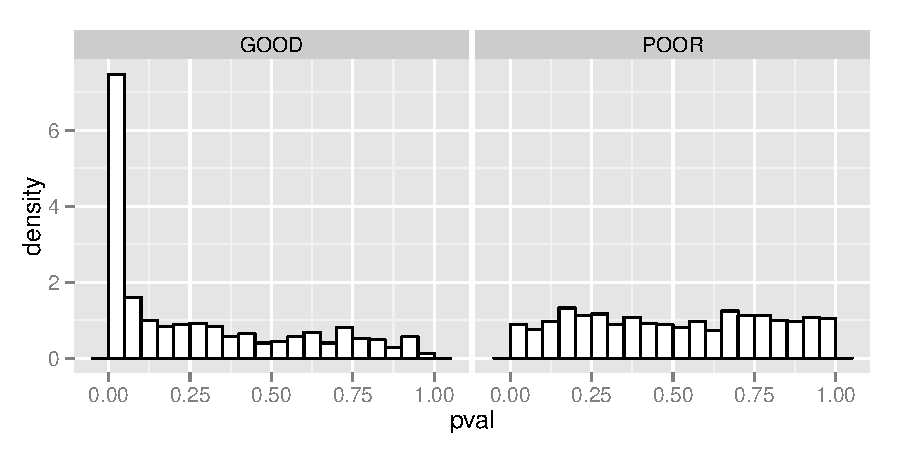
\includegraphics[height=3in]{Rcode/figures/good_poor_hist.pdf}
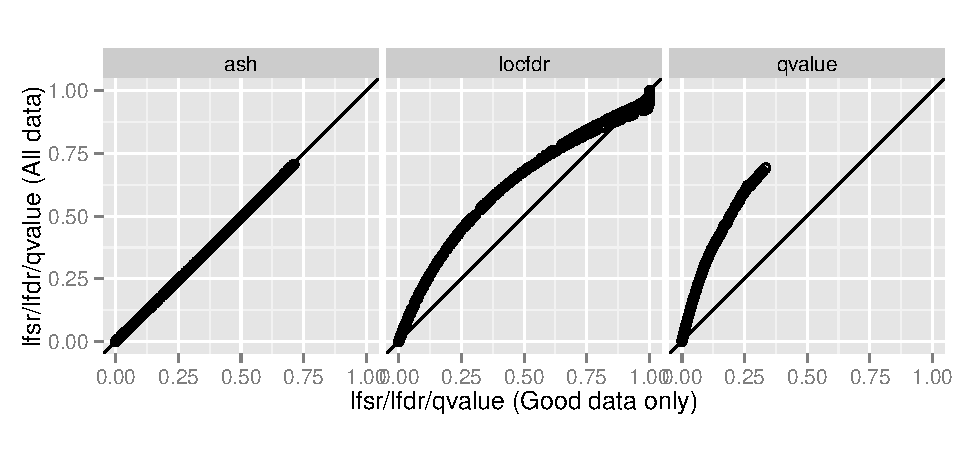
\includegraphics[width=6.5in]{Rcode/figures/good_vs_all.pdf}
\end{center}
\caption{}
\end{figure}


\subsection*{Improved conservative estimation of $\pi_0$}

To illustrate estimation of $\pi_0$ we provide simulation results for two scenarios:
\begin{enumerate}
\item[Scenario 1:]
\begin{equation}
f_1(\cdot) =  0.4 N(0,0.25^2) + 0.2 N(0,0.5^2) + 0.2 N(0,1^2), 0.2 N(0,2^2)
\end{equation}
\item[Scenario 2:]
\begin{equation}
f_1(\cdot) = N(0,4^2)
\end{equation}
\end{enumerate}
Scenario 1 represents a ``difficult" case where many non-zero $\beta$ are
too close to  zero to be reliably detected, making reliable estimation of $\pi_0$ essentially impossible; 
Scenario 2 represents an ``easier" case where most non-zero $\beta$ are
sufficiently different from zero that they can be reliably detected. making estimation of $\pi_0$ easier.
For Scenario 1 we considered datasets of size $n=1000$ (Scenario 1a) and $n=10,000$ (Scenario 1b);
for Scenario 2 we used $n=1000$.

For each simulation scenario we simulated 200 independent data sets. For each data set we simulated
the true value of $\pi_0  \sim U[0,1]$, and then simulated $\beta_j \sim \pi_0 \delta_0 + (1-\pi_0) f_1(\cdot)$
and $\bhat_j | \beta_j = N(\beta_j,1)$ for $j=1,\dots,n$. Thus these simulations assume the same
precision for each measurement. We applied the methods implemented in the R packages qvalue, fdrtool, locfdr, and mixfdr
for estimating $\pi_0$. We also applied our method to estimate $\pi_0$ in two ways, one using a penalty encourage
$\pi_0$ to be as large as possible (``null-biased"), and the other using the maximum likelihood estimate for $\pi$.


Figure \ref{fig:pi0} compares estimated and true values of $\pi_0$ under each Scenario. 
For Scenario 1, no method reliably estimates $\pi_0$. This is expected since, the scenario was designed to make accurate estimation
of $\pi_0$ impossible. However, we see that all the methods except for ash (mle) are able to provide a conservative
estimate for $\pi_0$. Further, among these the estimates from ash (null-biased) are least conservative. Scenario 2 produces similar patterns,
except that for this scenario the ash estimates of $\pi_0$ are quite accurate (made possible by the fact that most non-zero effects
are very different from zero).

These simulations illustrate two key points: i) although $\pi_0$ is not identifiable, the penalized likelihood approach
provides conservative estimates for $\pi_0$; ii) replacing the ``zero assumption" with the unimodal assumption can produce
less conservative, more accurate, estimates of $\pi_0$ (provided of course that the unimodal assumption holds, as it does in these simulations).

\begin{figure}[!ht] \label{fig:pi0}
\begin{center}
\includegraphics[height=160px,width=540px]{Rcode/figures/estpi0_sim1sim2.png}
\end{center}
\caption{Comparison of true and estimated values of $\pi_0$ for simulation scenarios. Scenarios 1a and 1b represent ``difficult" scenarios where $\pi_0$ is impossible to estimate accurately. However, all methods except the ash mle method are successful in providing conservative estimates for $\pi_0$. The ash (null-biased) method is least conservative, and hence most accurate, due to its additional assumption that the effect size distribution $g$ is unimodal.}
\end{figure}

Note that, even though the exact value of the point mass $\pi_0$ cannot, in general, be reliably estimated, the actual underlying distribution $g$ 
can be quite accurately estimated from the data, provided we assess accuracy by a metric that is not sensitive to $\pi_0$: for example
by measuring the difference between the true and estimated cumulative distribution function (cdf). See supplementary Figure \ref{} for examples.

\subsection*{Local False Sign Rate}

There are two reasons to use the lfsr instead of the lfdr: it is more generally meaningful (e.g. it applies
whether or not zero effects exist),  and estimation of lfsr is more robust to modeling assumptions and estimation of $\pi_0$. 
To illustrate this, we compared estimated and true values of both lfdr and lfsr for the simulated data (where the true
values are computed by Bayes Theorem using the true value of $g$ FILL IN THESE DETAILS?). 



\begin{figure}[!ht]
\begin{center}
\includegraphics[height=320px,width=540px]{Rcode/figures/lfsdr_sim1sim2_blowup.png}
\end{center}
\caption{Figure showing lfsr is more robust than lfdr}
\end{figure}

- Illustration that estimated lfsr is more robust.

- Illustration that adjusted estimate of lfsr is still more robust..

- Compare estimated lfsr with true lfsr for difficult simulation case, to show nearly achieves Bayes Risk?

\subsection{Accounting for measurement precision improves estimates of FDR/fsr}
 
- Illustration of effects of contamination on FDR by low-quality data
comparison with ash.



\subsection{Comparison of different underlying component distributions}

We simulated data under three scenarios for the underlying effect size distribution $g$:
\begin{enumerate}
\item[Scenario A:]
A mixture of zero-centered normals,
\begin{equation}
g(\cdot) =  (2/3) N(\cdot; 0,1) + (1/3) N(\cdot; 0, 2^2)
\end{equation}
\item[Scenario B:]
A symmetric ``flat-topped" distribution, designed to be difficult to capture by a mixture of zero-centered normals 
\begin{equation}
g(\cdot) = (1/7) [N(\cdot; -1.5, 0.5^2) + N(\cdot; -1, 0.5^2) + N(\cdot; 0.5, 0.5^2) + N(\cdot; 0, 0.5^2) + N(\cdot; 0.5, 0.5^2) + N(\cdot; 1, 0.5^2) + N(\cdot; 1.5, 0.5^2)]
\end{equation}
\item[Scenario C:]
An asymmetric distribution, 
\begin{equation}
g(\cdot) = (1/4) N(\cdot; -2 ,2^2) + (1/4) N(\cdot; -1 ,1.5^2) + (1/3) N(\cdot; 0 ,1) + (1/6) N(\cdot; 1,1) 
\end{equation}
\end{enumerate}
In each case we simulated $\bhat_j  = \beta_j + N(0,s^2_j=1)$.

Because the mixture of zero-anchored uniforms is more flexible than the mixture of zero-centered uniforms, which is more flexible
than the mixture of zero-centered normals, we expect that the likelihoods will satisfy $L_{hu} > L_u > L_n$. However, for Scenario A we expect the differences in
likelihood to be small, because the true model here is a mixture of zero-centered normals, so any gain of $L_{hu}$ and $L_u$ over $L_n$ is necessarily due to ``overfitting".
For Scenario B, we expect that $L_{hu}$ and $L_{u}$ to be significantly larger than $L_n$, but any 
increase of $L_{hu}$ over $L_u$ must be due to overfitting (because the truth is symmetric). Finally, for Scenario C we
expect $L_{hu}$ to be significantly larger than the others.

Figure \ref{fig:rmse_loglik_boxplot} illustrates this.


\begin{figure}[!ht] \label{fig:rmse_loglik_boxplot}
\begin{center}
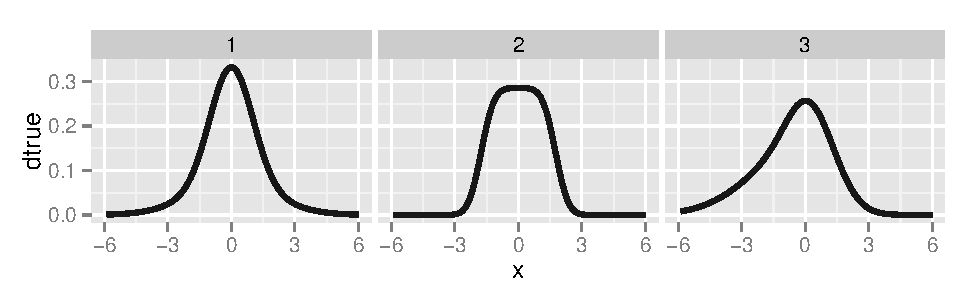
\includegraphics[width=6.5in]{Rcode/figures/simABC_egdens.pdf}
%\includegraphics[width=6.5in]{Rcode/figures/rmse_loglik_boxplot.pdf}
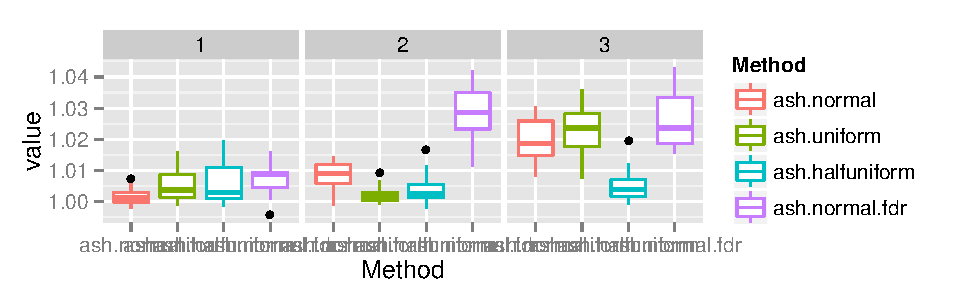
\includegraphics[width=6.5in]{Rcode/figures/rmse_boxplot.pdf}
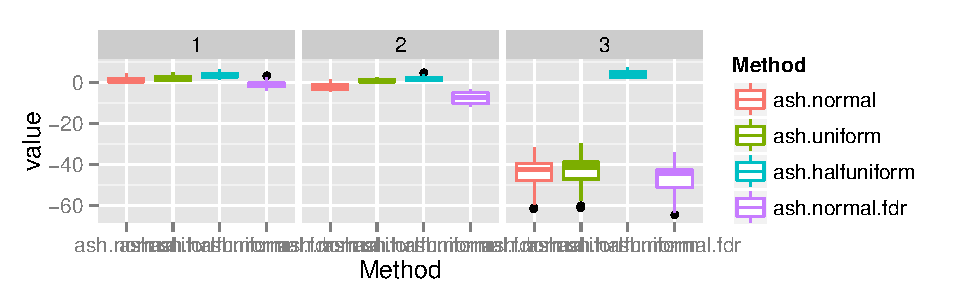
\includegraphics[width=6.5in]{Rcode/figures/loglik_boxplot.pdf}
\end{center}
\caption{}
\end{figure}

- how does use of the VB approach to estimate pi affect RMSE?

- Comparison between exchangeable effects vs Exchangeable standardized effects; Hedenberg data. 

- Possibly difference between CIs obtained by ash and usual CIs (e.g. ``of intervals where local fsr is <0.05, what proportion are the sign correct"?).


- Asymmetric case (Half uniforms)

Things to emphasise for paper:
- the number of components is not critical; the unimodal constraint is enough. You can increase the number of components arbitrarily and the likelihood remains bounded.
- the ability to incorporate item-specific measurement error
- the ability to compare a model in which effects are proportional to error
with model in which effects 

- bayesian coverage intervals (attempt to) give much stronger guarantess than standard confidence intervals. Eg among the 0.95 intervals excluding 0,
less than 5% should actually be 0?

Some advantages of the unimodal constraint:
-more statsitically efficient (if true); show with small sample sizes.
- less sensitive to number of components? Can allow number to tend to infinity?
- may be less sensitive to local optima?
could demonstrate this by looking at convergence more carefully, and comparing
results with random starting points.

- it allows us to easily just vary sigma on a grid, and fit pi, which
makes allowing different noise levels really easy!




\subsection{The number of components is not critical}
OR - this section could be more generally about selecting between
models (normal, uniforms etc) using log-likelihood.

Because of the uni-modal constraint, the number of mixture components
is generally not critical, at least provided it is ``sufficiently large". 
Indeed, as the number of components tends to infinity, the likelihood
is bounded above, and even for large numbers of components and small amounts of data the inferred underlying distributions tend not to be too crazy, showing few signs of ``overfitting". 

However, it is true that the normal distributions tend to yield smoother estimated underlying distributions. Similarly, using the posterior mean for $\pi$, rather
than the maximum likelihood estimate, tends to lead to somewhat smoother fitted distributions. In addition, with small amounts of data the underlying
distributions are inevitably not well determined by the data, and the fits may vary depending on the underlying assumptions made (e.g. number of components or distribution of the components); however, even then shrinkage-based estimates
of the betas can be relatively robust.

\subsection{Do we need a point mass at zero?}

In some settings it is the convention to focus on testing whether $\beta_j=0$. However some dislike this focus, objecting that it is unlikely to be the case that $\beta_j=0$ exactly. For example, when comparing the average expression of a gene in human samples vs chimp samples, it might be considered unlikely that the expression
is *exactly* the same in both. Whether or not $\beta_j=0$
is considered unlikely may depend on the context.
However, in most contexts, finite data cannot
distinguish between $\beta_j=0$ and $\beta_j$ being very close to zero. Thus finite data cannot usually convince a skeptic that $\beta_j$ is exactly zero, rather than just very small. In contrast it is easy to imagine data that would convince a doubter that $\beta_j$ is truly non-zero. In this sense there is an assymetry between the inferences "$\beta_j$ is zero" and "$\beta_j$ is non-zero", an assymetry that is reflected in the admonition "failure to reject the null does not imply it to be true".

Thus any analysis that purports to distinguish between these cases must be making an assumption. 

Consider two analyses of the same data, using two different "priors" $g$ for $\beta_j$, that effectively differ only in their assumptions about whether or not $\beta_j$ can be exactly zero. For concreteness, consider
\[ g_1(\cdot) = \pi \delta_0(\cdot) + (1-\pi) N(\cdot; 0,\sigma^2) \]
and
\[g_2(\cdot) = \pi N(\cdot; 0, \epsilon^2) + (1-\pi) N(\cdot; 0, \sigma^2).\]
If $\epsilon^2$ is sufficiently small, then these 
priors are "approximately the same", and will lead to "approximately the same" posteriors and inferences in many senses. To discuss these, let $p_j$ denote the posterior under prior $g_j$. Then, for any given (small) $\delta$, we will have $p_1(|\beta_j|<\delta) \approx p_2(|\beta_j|< \delta)$. However, we will not have $p_1(\beta_j=0) \approx p_2(\beta_j=0)$: the latter will always be zero, while the former could be appreciable.

 What if, instead, we examine $p_1(\beta_j >0)$ and $p_2(\beta_j >0)$? Again, these will differ. If this probability is big in the first analysis, say $1-\alpha$ with $\alpha$ small, then it could be as big as $1-\alpha/2$ in the second analysis. This is because if $p_1(\beta_j>0)=1-\alpha$, then $p_1(\beta_j=0)$ will often be close to $\alpha$, so for small $\epsilon$ $p_2(\beta_j)$ will have mass $\alpha$ near 0, of which half will be positive and half will be negative. 
Thus if we do an analysis without a point mass, but allow
for mass near 0, then we may predict what the results would have been if we had used a point mass.

Let's try: 
```{r}
beta.ash.pm = ash(ss$betahat, ss$betasd, usePointMass=TRUE)
print(beta.ash.pm)
print(beta.ash.auto)
plot(beta.ash.auto$localfsr,beta.ash.pm$localfsr,main="comparison of ash localfsr, with and without point mass",xlab="no point mass", ylab="with point mass",xlim=c(0,1),ylim=c(0,1))
abline(a=0,b=1)
abline(a=0,b=2)
```

Our conclusion: if we simulate data with a point mass,
and we analyze it without a point mass, we may underestimate
the lfsr by a factor of 2. Therefore, to be conservative, we might prefer to analyze the data allowing for the point mass, or, if analyzed without a point mass, multiply estimated false sign rates by 2. In fact the latter might be preferable: even if we analyze the data with a point mass, there is going to be some unidentifiability
that means estimating the pi value on the point mass will be somewhat unreliable, and we still might underestimate the false sign rate if we rely on that estimate.  
TO THINK ABOUT: does multiplying the smaller of Pr(<0) and Pr(>0) by 2, and adding to Pr(=0) solve the problem in either case?


\subsection{Side notes on Multiple comparisons}

Note on multiple comparisons: it isn't really a "problem" but an "opportunity". This viewpoint also espoused by Greenland and Robins. It isn't the number of tests that is relevant (the false
discovery rate at a given threshold does not depend on the number of tests). It is the *results* of the tests that are relevant.

Performing multiple comparisons, or multiple tests, is often
regarded as a "problem". However, here we regard it instead as an opportunity - an opportunity to combine (or "pool") information across tests or comparisons.

Imagine that you are preparing to perform 1 million tests,
each based on a $Z$ score that is assumed to be $N(0,1)$ under the null.
You first order these tests randomly, and begin by 
performing the first test, which returns a $Z$ score of 4.
At this point you are interrupted by a friend, who asks how the analysis is going. "It's early days, but looking promising" you reply. Well, who wouldn't? If the aim is to find lots of significant differences, a strong first result is surely a good outcome. 

At this point you have reason to expect that many of the
subsequent tests also output strong results.

Now consider two alternative scenarios for the remaining 999,999 tests. In the first scenario, the remaining tests
produce $Z$ values that fit very well with the null, closely following a standard normal distribution; in the second
scenario a large proportion of the remaining tests, say 50 percent, show outcomes that lie outside of $[-4,4]$. 

If your friend enquired after your analysis again, your
response would surely differ in the first scenario ("Oh, it didn't pan out so well after all") vs the second ("It went great"). Further,
in the first scenario, if your friend pressed you further about the results of the first test,
you would likely, I think, be inclined to put them down to chance. In contrast, in the second scenario, the first test turned out to be, as you hoped, a harbinger of good things to come, and in this scenario you would likely regard that test as likely corresponding to a true discovery.

The key point is that it is the *outcomes* of the tests, not the *number* of tests, that impacts interpretation of that first test. 

(Some may by pondering whether the fact that you are about to perform another
999,999 tests should be considered pertinent in responding to your friend. Our view is that it is  irrelevant.
The standard frequentist framework would disagree, because
it requires the analyst to consider hypothetical repetitions
of the "experiment", and so the fact that the experiment
consists of a million tests is pertinent. However, this
argument is a distraction from the main point.)

Indeed, we believe that the practice of focussing on the *number* of tests performed is 

Focussing on the number of tests performed can be
seen as an approximation. 

The standard argument is that,
when performing multiple tests, some will be significant
just by chance.

\subsection{Discussion}

Efron (2008) states the Zero Assumption as the assumption that ``most of the z-values near zero come from null genes".
His main aim in making this assumption is to estimate an empirical null though (not assume N(0,1) for the null)
rather than to impose identifiability.

Note that \cite{muralidharan:2012} models $z$ scores as something plus noise under both $H_0$ and $H_1$, which
avoids this problem. (DOes the same maybe apply to modeling beta, rather than z scores, when the errors vary?)

Rice and Spiegelhalter - BRCA data?

A fundamental idea is
that the measurements of $\beta_j$ for each gene can be used to improve inference for the values of $\beta$ for other genes.


% Do NOT remove this, even if you are not including acknowledgments
\section*{Acknowledgments}

Statistical analyses were conducted in the {\sf R} programming language \cite{Rcore:2012}, Figures produced using the ggplot2 package \cite{ggplot2}, and text
prepared using \LaTeX.

%\section*{References}
% The bibtex filename
\bibliography{/Users/stephens/Documents/mainbib}

\section*{Figure Legends}


\clearpage

\section*{Tables}

\section*{Supporting Information Legends}

Supplementary material can be found in {\bf Supplementary Information S1.}
%\begin{table}[!ht]
%\caption{
%\bf{Table title}}
%\begin{tabular}{|c|c|c|}
%table information
%\end{tabular}
%\begin{flushleft}Table caption
%\end{flushleft}
%\label{tab:label}
% \end{table}

\end{document}

